\documentclass{article}

\usepackage{polski}
\usepackage[UTF8]{inputenc}
\usepackage{graphicx}
\usepackage{float}
\usepackage[margin=1in]{geometry}
\usepackage{graphicx}
\usepackage{amsmath}
\usepackage{mathtools}
\usepackage{amssymb}
\usepackage{multirow}
\usepackage{changepage}
\usepackage{pbox}
\usepackage{siunitx}
\usepackage{enumerate}

\title{Sprawozdanie}
\begin{document}
\begin{center}
\bgroup
\def\arraystretch{1.5}
\begin{tabular}{|c|c|c|c|c|c|}
	\hline
	EAIiIB & \multicolumn{2}{|c|}{\begin{tabular}{@{}c@{}}Autor 1 \\ Autor 2\end{tabular}} & Rok II & Grupa 5 & Zespół 6 \\
	\hline
	\multicolumn{3}{|c|}{\begin{tabular}{c}Temat: \\ Elektroliza \end{tabular}} & 
	\multicolumn{3}{|c|}{\begin{tabular}{c}Numer ćwiczenia: \\ 35 \end{tabular}} \\
	\hline
	 Data wykonania & Data oddania & Zwrot do poprawki & Data oddania & Data zaliczenia & Ocena \\[6ex]
	\hline
\end{tabular}
\egroup
\end{center} 

%WSTEP
\section{Cel ćwiczenia}
Wyznaczenie stałej Faradaya oraz równoważnika elektrochemicznego miedzi metodą elektrolizy.

\section{Wstęp teoretyczny}
\subsection{Elektrolity i dysocjacja elektrolityczna}
\textit{Elektrolity} są to wodne roztwory kwasów zasad i soli. Są to substancje krystaliczne które po rozpuszczeniu przechodzą do roztworów w postaci jonów, proces ten nazywamy \textit{dysocjacją elektrolityczną}. Gdy do roztworu wstawimy elektrody i dołączymy je do źródła prądu stałego ruch jonów staje się uporządkowany. Na elektrodach jony zostają zobojętnione wynikiem czego jest wydzielanie się substancji na elektrodach. Liczba atomów wydzielonych na elektrodzie jest równa stosunkowi wartości dostarczonego ładunku do ładunku pojedynczego jonu:
$$ N = \frac{It}{we} $$

\subsection{Prawa elektrolizy Faradaya}
\begin{enumerate}[I]
	\item Masa $m$ substancji wydzielonej na elektrodzie jest proporcjonalna do natężenia prądu $I$ oraz do czasu jego przepływu $t$: $$ m = kIt $$ Współczynnik proporcjonalności $k$ to tak zwany równoważnik elektrochemiczny substancji.
	
	\item Równoważniki elektrochemiczne $k$ pierwiastków są proporcjonalne do ich równoważników chemicznych $\frac{\mu}{w}$.
	$$F = \frac{\mu}{wk} $$
	Współczynnik proporcjonalności $F$ to stała Faradaya. Jej tabelaryczna wartość to $F = 96500\ \mbox{[C]}$.
\end{enumerate}

\section{Układ pomiarowy}
Zestaw ćwiczeniowy stanowi naczynie do elektrolizy siarczanu miedzi $CuSO_{4}$ z miedzianymi elektrodami w kształcie równoległych płyt, oddalonych od siebie o kilka centymetrów, zasilacz napięcia stałego, amperomierz, waga elektroniczna.
\begin{figure}[!htb]
	\centering
	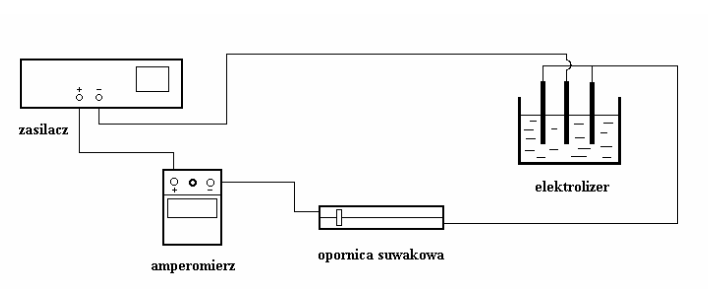
\includegraphics[scale=0.65]{obwod.png}
	\caption{Schemat obwodu elektrycznego}
\end{figure}	
\section{Wykonanie ćwiczenia}
Doświadczenie zostało wykonane za pomocą obwodu elektrycznego przedstawionego na rysunku. Elektrody wykonane zostały z miedzi, zewnętrze pełnią rolę anod, natomiast elektroda wewnętrzna katody. Po uprzednim oczyszczeniu i zważeniu elektrody zostały zanurzone w elektrolicie, którym jest wodny roztwór siarczanu miedzi $CuSO_{4}$. Elektroliza przebiegała przez $t = 30$ min., natężenie prądu płynącego w obwodzie wynosiło $I = 0,7$\mbox{[A]}.
	

%KONIEC WSTEPU	

\section{Opracowanie wyników}
\subsection{Obliczenia}
\begin{enumerate}
	\item Masa miedzi wydzielonej podczas elektrolizy na katodzie:
	\begin{align*} m = 408\ \mbox{[mg]}\end{align*}
	\item Zmiana masy anod podczas elektrolizy.
	\begin{align*} m_{1} = 215\ \mbox{[mg]} \\
	 m_{2} = 209\ \mbox{[mg]}\end{align*}
	\item Obliczamy wartość równoważnika elektrochemicznego miedzi korzystając z pierwszego prawa elektrolizy Faradaya.
	\begin{align*} k = \frac{m}{It} = 0,323\ \left [\frac{mg}{C} \right ]\end{align*}
	\item Korzystając z drugiego prawa elektrolizy Faradaya i otrzymanego równoważnika elektrochemicznego $k$ liczymy stałą Faradaya.
	\begin{align*} & \mu = 63,58\ \left[\frac{g}{mol} \right ] \\ & w = 2 \\ & F = \frac{\mu}{kw} = 98174\ \left[\frac{C}{mol} \right ] \end{align*}
	\item Wyznaczamy wielkość ładunku elementarnego z obliczonej stałej Faradaya.
	\begin{align*}e = \frac{F}{N_{A}} = \frac{98174}{6,022\cdot 10^{23}} = 1,6302 \cdot 10^{-19}\ \mbox{[C]} \end{align*}
\end{enumerate}
\pagebreak
\subsection{Obliczenie niepewności pomiarowych}
\begin{enumerate}
	\item Niepewność wagi elektronicznej wynosi $ 0,001\ \mbox[g] $.
	\item Niepewność pomiaru wydzielonej masy miedzi przyjmujemy jako:
$$ u(m) = 0,01\ \mbox{[g]}$$
Związane jest to z możliwością niedokładnego przepłukania lub wysuszenia miedzi.
	\item Niepewność pomiaru natężenia prądu:
$$ u(I) = \frac{K \cdot Z}{100} = \frac{0,5 \cdot 0,75}{100} = 3,75\ {[mA]}$$
	\item Niepewność pomiaru czasu pomijamy, ponieważ jest ona zaniedbywalnie mała względem pozostałych \\niepewności.

	\item Niepewność pomiaru ładunku, który przepłynął przez elektrolit:
$$u(Q) = u(I)\cdot t = 0,375 \cdot 1800 = 6,75\ [C] $$
	\item Niepewność równoważnika elektrochemicznego miedzi:
	\begin{equation*}
		u(k) = \sqrt{\bigg(\frac{\partial k}{\partial m}u(m)\bigg)^2+\bigg(\frac{\partial k}{\partial I}u(I)\bigg)^2+\bigg(\frac{\partial k}{\partial t}u(t)\bigg)^2} =	\sqrt{\bigg(\frac{1}{It}u(m)\bigg)^2+\bigg(\frac{m}{I^{2}t}u(I)\bigg)^2+\bigg(\frac{m}{It^{2}}u(t)\bigg)^2} = 8,123 \ \left [\frac{ \mu g }{C} \right ]
	\end{equation*}
	\item Niepewność wyznaczenia stałej Faradaya:
$$u(F)=F \frac{u(k)}{k} = 2463,06\ \mbox{[C]}$$
	\item Niepewność wyznaczenia ładunku elementarnego:
$$u(e) = \sqrt{(\frac{\partial e}{F}u(F))^2} = \frac{1}{N_{A}}u(F) = 4,0901 \cdot 10^{-21}\ \mbox{[C]} $$
\end{enumerate}
\begin{figure}[H]
	\begin{adjustwidth}{-1cm}{}
\def\arraystretch{1.3}
\centering
	\begin{tabular}{|c|c|c|c|c|c|c|}
		\cline{2-7}
		 \multicolumn{1}{c|}{} & \begin{tabular}{c}Wartości \\tablicowe\end{tabular}& \begin{tabular}{c}Wartości \\otrzymane\end{tabular} & Różnica& \begin{tabular}{c}Niepewność \\standardowa\end{tabular} & \begin{tabular}{c}Niepewność \\ rozszerzona \\ $k=2$ \end{tabular} & \begin{tabular}{c}Zgodność z \\ wartością tablicową \\ $|x - x_{0}| < U(x)$ \end{tabular}\\
		\hline
		$k$ \mbox{[$\frac{\mu g}{C}$]} & 329 & 323 & 6 & 8,123 & 16,246 & Tak  \\
		\hline
		$F$ \mbox{[$C$]} & 96500 & 98174 & 1674 & 2463 & 4926 & Tak \\
		\hline
		$e$ \mbox{[$C$]} & $1,6021 \cdot 10^{-19}$ & $1,6302 \cdot 10^{-19}$ & $7,2334 \cdot 10^{-24}$& $4,0901 \cdot 10^{-21}$ & $8,1802 \cdot 10^{-21}$ & Tak \\
		\hline	
	\end{tabular}
\end{adjustwidth}
\end{figure}
 
 \section{Wnioski}
	Po obliczeniu niepewności rozszerzonej stwierdzamy, że wszystkie wyznaczone stałe:
	\begin{itemize}
		\item równoważnik elektrochemiczny miedzi
		\item wartość ładunku elementarnego
		\item stała Faradaya
	\end{itemize}
	 są zgodne z wartościami tablicowymi.
	
\end{document}